%% ============================================================
%%  Enhanced Mobility Device with Proximity Sensors Technology
%%  Tsotlhe Seiphepi, Adamu Murtala Zungeru, Jwaone Gaboitaolelwe
%%  Botswana International University of Science and Technology
%% ============================================================
\documentclass[12pt, a4paper]{article}

% ---- Packages -----------------------------------------------
\usepackage[T1]{fontenc}
\usepackage[utf8]{inputenc}
\usepackage{lmodern}
\usepackage[margin=2.5cm]{geometry}
\usepackage{graphicx}
\usepackage{amsmath}
\usepackage{amssymb}
\usepackage{siunitx}
\usepackage{booktabs}
\usepackage{array}
\usepackage{float}
\usepackage{subcaption}
\usepackage[hidelinks]{hyperref}
\usepackage{cite}
\usepackage{titlesec}
\usepackage{abstract}
\usepackage{setspace}
\usepackage{microtype}
\usepackage{parskip}

% ---- Path for figures ----------------------------------------
\graphicspath{{figures/}}

% ---- Section formatting --------------------------------------
\titleformat{\section}{\large\bfseries}{\Roman{section}.}{0.75em}{}
\titleformat{\subsection}{\normalsize\bfseries\itshape}{\Roman{subsection}.}{0.75em}{}
\titleformat{\subsubsection}{\normalsize\itshape}{\roman{subsubsection}.}{0.75em}{}

% ---- Abstract style ------------------------------------------
\renewcommand{\abstractnamefont}{\normalfont\itshape}
\renewcommand{\abstracttextfont}{\normalfont\itshape}
\setlength{\absleftindent}{2cm}
\setlength{\absrightindent}{2cm}

% ---- Document ------------------------------------------------
\begin{document}

\begin{titlepage}
    \centering
    \vspace*{2cm}
    {\Large\bfseries ``Enhanced Mobility Device with Proximity Sensors Technology.''\par}
    \vspace{1.5cm}
    {\normalsize
        Tsotlhe Seiphepi, Adamu Murtala Zungeru, Jwaone Gaboitaolelwe\par
        \vspace{0.4cm}
        Department of Electrical, Computer and Telecommunications Engineering,\\
        Botswana International University of Science and Technology\\
        Private Bag 16, Palapye, Botswana\par
    }
    \vspace{2cm}
    \hrule
    \vspace{1cm}
    \begin{abstract}
        Navigating environments poses substantial challenges for visually impaired
        individuals due to the rapid changes in their surroundings, making memorization
        difficult and increasing the risk of serious injury. This dependency on assistance from
        others highlights the limitations of traditional aids like walking canes, which require
        physical contact with obstacles and have a limited detection range of usually 1 metre.
        Moreover, using walking canes demands significant mental mapping of the
        surroundings and constant attention to tactile feedback. This paper presents the
        design and simulation of an Enhanced Mobility Device using Proximity Sensors,
        aimed at improving navigation for visually impaired individuals. The proposed device
        is a stick integrated with HC-SR04 proximity sensors and NE555 timers, which detect
        objects and alert the user through DC-operated motors that provide vibrations. This
        system is designed to enable users to better navigate their surroundings without the
        need for constant physical contact or intensive mental mapping. The circuit was
        designed, simulated, and tested in Proteus simulation software, yielding positive
        results. The Enhanced Mobility Device demonstrates significant potential to reduce
        dependency on others, increase safety, and provide a more efficient means of
        navigation for visually impaired individuals.
    \end{abstract}
    \vspace{0.5cm}
    \hrule
    \vspace{1cm}
    \noindent\textbf{Keywords:} Object Detection; Proximity Sensor (HC-SR04); NE555 Timer; DC Motor.
\end{titlepage}

% =============================================================
\section{Introduction}
% =============================================================

Blind individuals often face significant challenges navigating their surroundings without secondary
human assistance, particularly in unfamiliar environments where obstacles are not easily detectable.
Traditional walking aids such as canes and walking stands have significant limitations. To address this
critical need for enhanced mobility and safety, various technological advancements have been developed,
including Smart Glasses for the Visually Impaired~\cite{ali2016smart}. These glasses use recognition
technology and convert it into auditory feedback, thereby assisting visually impaired users in
interpreting their surroundings, which is achieved through image processing techniques. Another
revolution is the LiDAR-Based Obstacle Detection and Distance Estimation in Navigation Assistance
for the Visually Impaired~\cite{lidar2020}, of which EfficientDet-LiteV4 is used for obstacle detection,
and a depth map from the LiDAR is used to estimate object distance to different obstacles.

Augmented Reality Navigation Systems For The Blind~\cite{kuriakose2021navigation} convert physical
environments to digital information. This system combines cameras and sensors including software
algorithms to create a detailed overview of the users' surroundings to provide navigational assistance
through auditory feedback. Advancement of haptic aids, such as the Haptic Navigation Aid for Spatial
Perception, led to the creation of The OptiBand, a wearable haptic navigation device designed to
enhance spatial awareness for blind and visually impaired individuals. Equipped with LiDAR sensors,
it detects objects up to 15 metres away and communicates their presence and location through haptic
feedback~\cite{ojeda2023optiband}. The Smart Shoes Safety System for the Blind based on Internet of
Things (IoT) Technology incorporates three ultrasonic sensors and a microprocessor to detect obstacles
and measure distances, alerting the user through auditory signals when an obstacle is near. The system
also includes water and flame sensors for detecting potential hazards and uses GPS
technology~\cite{almomani2023smart}.

Developing a proximity sensor stick for the blind incorporates these advancements by providing
real-time feedback about obstacles in the user's path, significantly improving their quality of life. The
focus of this project is to design and develop a lightweight, portable, and user-friendly proximity sensor
stick capable of detecting obstacles up to 1~m, with a battery-rechargeable feature providing
non-intrusive feedback for individuals with varying degrees of visual impairment. Consideration has
been given to factors such as cost-effectiveness, durability, and ease of maintenance to ensure the
device's practical and widespread use, enabling blind individuals to navigate confidently and
independently in both indoor and outdoor settings.

% =============================================================
\section{Materials and Methods}
% =============================================================

This section provides an overview of the Enhanced Mobility Device's subsystems. Utilising proximity
sensors (HC-SR04), the device is designed to scan and detect objects within the user's path. The system
comprises six subsystems: power supply, sensor system, timing system, switching system, and feedback
or output system, as illustrated in Figure~\ref{fig:blockdiagram}.

\begin{figure}[H]
    \centering
    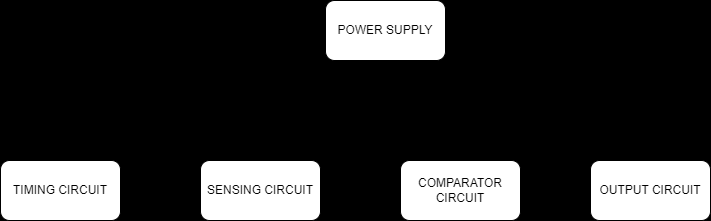
\includegraphics[width=0.85\textwidth]{fig01_block_diagram.png}
    \caption{Block diagram for the Enhanced Mobility Device using Proximity Sensors subsystems.}
    \label{fig:blockdiagram}
\end{figure}

\begin{figure}[H]
    \centering
    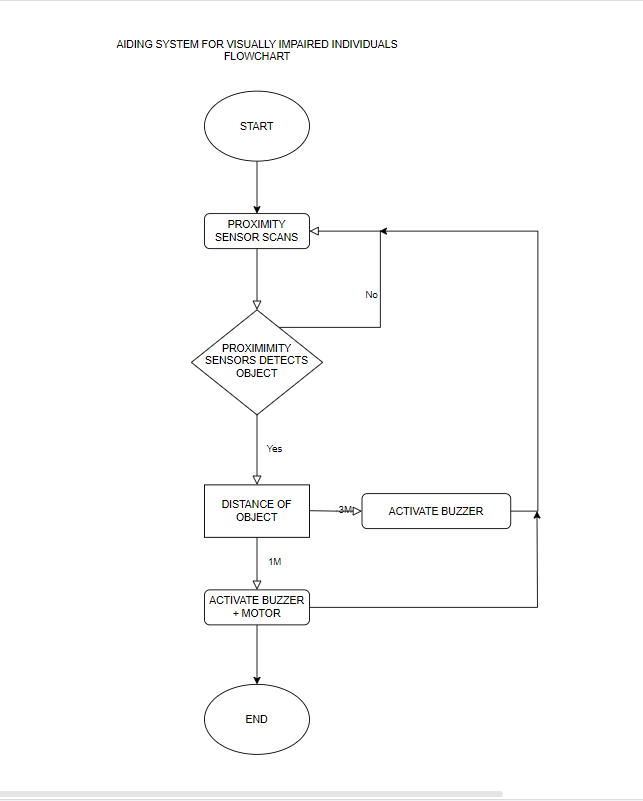
\includegraphics[width=0.72\textwidth]{fig02_flowchart.png}
    \caption{Flowchart for obstacle detection using the proposed design.}
    \label{fig:flowchart}
\end{figure}

% ----- I. Power Supply ----------------------------------------
\subsection{Power Supply}

The design is operated by a 9~V battery. It supplies the different sub-circuits: timing circuit,
comparator circuit, and the output circuit.

\begin{figure}[H]
    \centering
    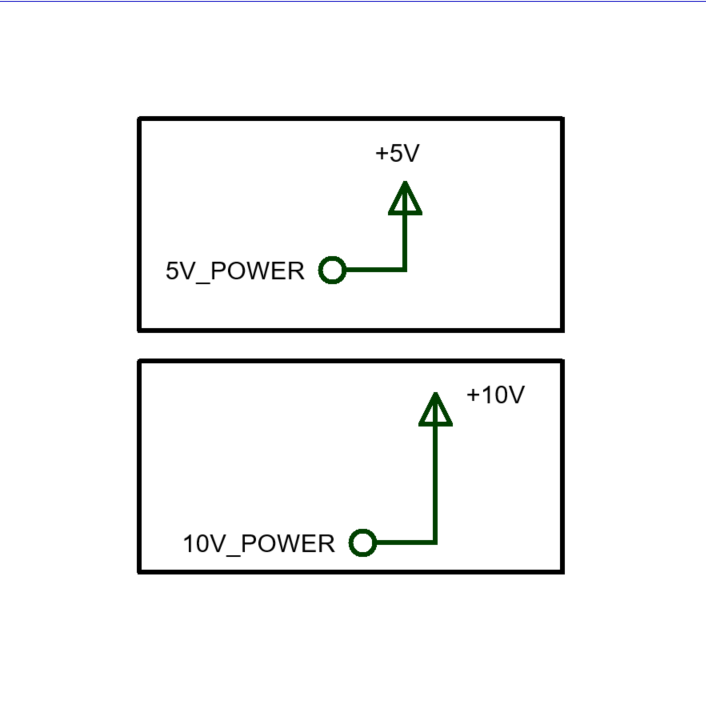
\includegraphics[width=0.55\textwidth]{fig03_power_supply.png}
    \caption{Diagram showing the power supply of the design.}
    \label{fig:powersupply}
\end{figure}

% ----- II. Sensory Circuit ------------------------------------
\subsection{Sensory Circuit}

The sensing circuit detects obstacles as the user is moving. For the design, the HC-SR04 ultrasonic
component is used. The HC-SR04 sensor functions by emitting an ultrasonic pulse and receiving the echo
of this pulse to measure distance. The primary components of an equivalent circuit include the trigger
mechanism, the pulse generator (transmitter), the receiver, and the control logic that processes the echo
time to determine distance. The ultrasonic distance measuring sensor is a non-contact distance
measurement device. The range of measuring distance is 2~cm to 400~cm, with a precision of 3~mm.
The internal structure of the HC-SR04 ultrasonic sensor mainly consists of three parts: the waveform
generator, the signal receiver, and the control circuit. The control circuit primarily includes
amplification, filtering, and shaping. The HC-SR04 sensor has four external I/O ports; the pin names
are VCC, GND, Trig, and Echo. When the Echo pin receives the transmitted signal, the change of the
pin becomes a high level, representing the success of a range measurement~\cite{lastminute2024}.

\begin{figure}[H]
    \centering
    \begin{subfigure}[t]{0.45\textwidth}
        \centering
        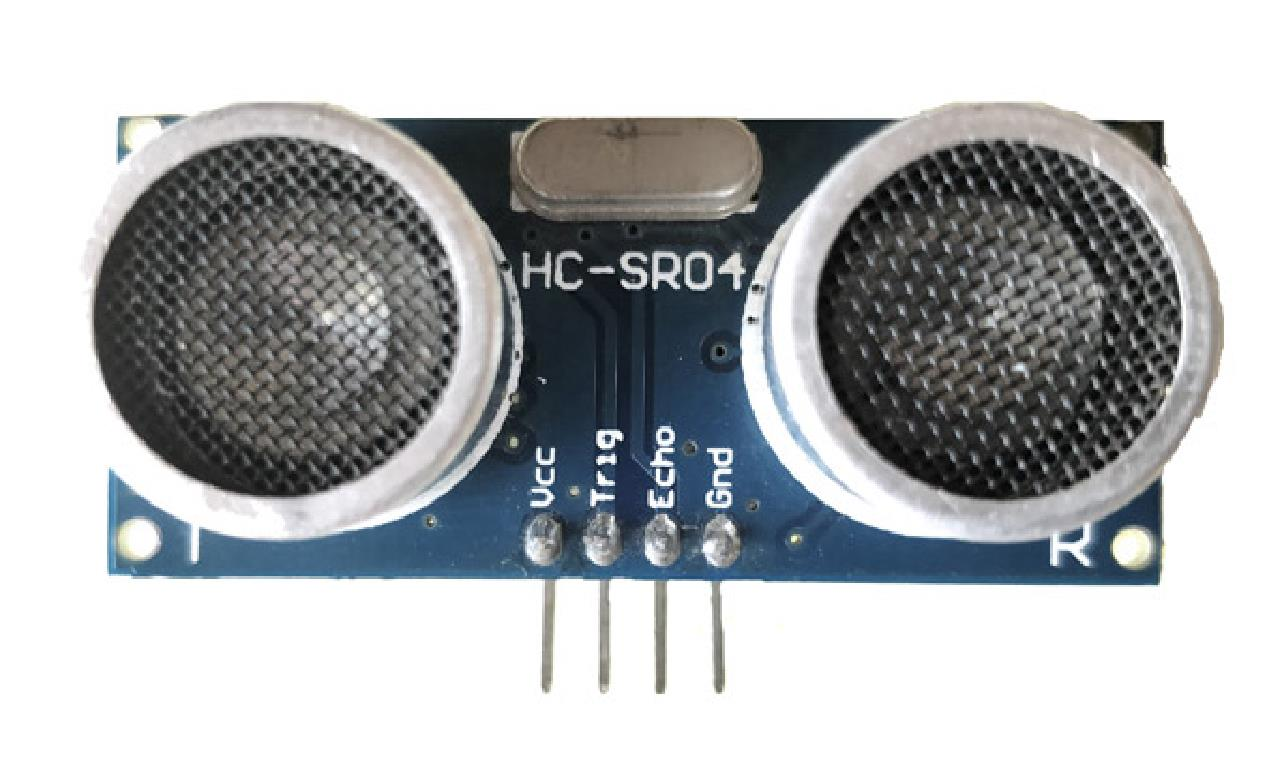
\includegraphics[width=\textwidth]{fig04a_hcsr04_sensor.jpeg}
        \caption{HC-SR04 proximity sensor.}
        \label{fig:hcsr04}
    \end{subfigure}
    \hfill
    \begin{subfigure}[t]{0.50\textwidth}
        \centering
        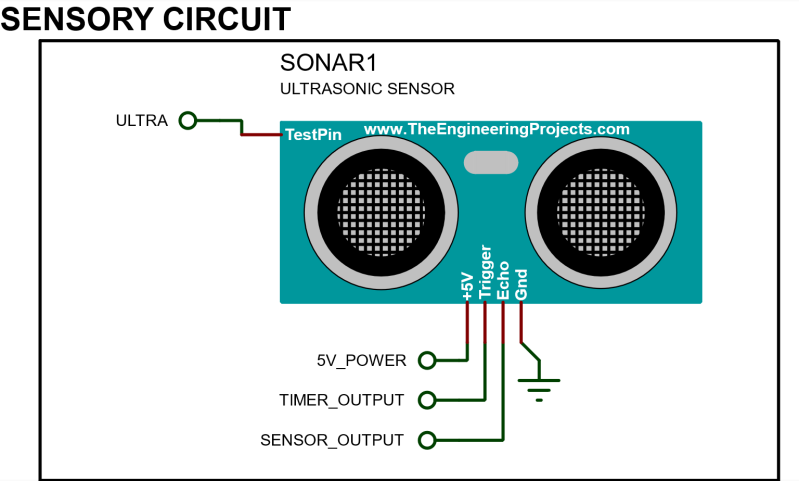
\includegraphics[width=\textwidth]{fig04b_sensory_circuit.png}
        \caption{Proteus image of the sensory circuit.}
        \label{fig:sensorcircuit}
    \end{subfigure}
    \caption{HC-SR04 sensor and its Proteus simulation circuit.}
    \label{fig:sensorgroup}
\end{figure}

% ----- III. Timing Circuit ------------------------------------
\subsection{Timing Circuit}

For the design, input signals from the sensory circuits are sampled at fixed intervals. Instead of
processing a single input, the system continuously scans and samples the surroundings for obstacles.
The proximity sensor (HC-SR04), operating at 250~Hz, is configured using the NE555 timer in its
astable mode to achieve the necessary functionality.

\subsubsection*{NE555 Timer in Astable Mode}

The NE555 Timer IC configured in Astable Mode functions as a free-running oscillator, meaning it
continuously generates a square wave output without requiring any external trigger. This mode is used
to create clock pulses and PWM (Pulse Width Modulation) signals~\cite{gui2018ultrasonic}.

\begin{figure}[H]
    \centering
    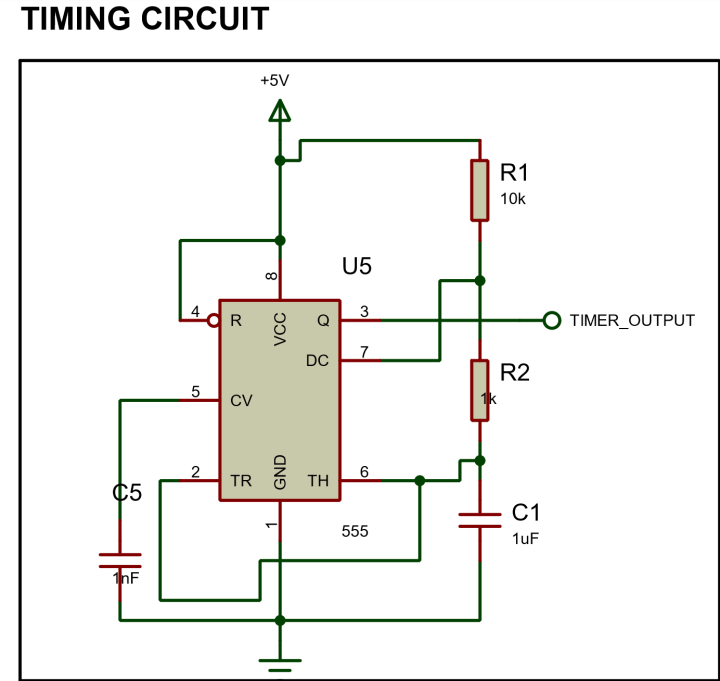
\includegraphics[width=0.65\textwidth]{fig05_timing_circuit.png}
    \caption{Internal diagram for the NE555 timer timing circuit.}
    \label{fig:timingcircuit}
\end{figure}

To achieve a time period of 2~seconds, the following calculations are completed to determine the values
of the capacitor and resistors $R_1$ and $R_2$:

\begin{equation}
    f = \frac{1.44}{(R_1 + 2R_2) \times C}
    \label{eq:freq}
\end{equation}

\begin{equation}
    T = \frac{1}{f}
    \label{eq:period}
\end{equation}

\begin{equation}
    T = (R_1 + 2R_2) \times C \times 1.44
    \label{eq:period2}
\end{equation}

where $f$ is the frequency of oscillation, $C$ is the capacitance in farads (F), and $R_1$, $R_2$ are
resistance values in ohms ($\Omega$).

\noindent\textbf{i. Frequency Setup:}

Given the desired frequency $f = 250$~Hz, the combined product of resistance and capacitance is
calculated as:

\begin{equation}
    (R_1 + 2R_2) \times C = \frac{1.44}{f} = \frac{1.44}{250\,\text{Hz}} = 0.576\,\text{s}
    \label{eq:rc}
\end{equation}

\noindent\textbf{ii. Capacitor Selection:}

\[
    C = 1\,\mu\text{F} \quad \text{(fixed value)}
\]

\noindent\textbf{iii. Resistor Selection:}

Choosing $R_A = 1{,}000\,\Omega$ to balance the circuit design, $R_B$ is calculated as:

\[
    1{,}000 + 2R_B = 36{,}000 \implies 2R_B = 35{,}000 \implies R_B = 17{,}500\,\Omega
\]

\noindent\textbf{iv. Frequency Verification:}

\begin{equation}
    f = \frac{1.44}{(1{,}000 + 2 \times 17{,}500) \times 0.000001} \approx 250\,\text{Hz}
    \label{eq:freqverify}
\end{equation}

Therefore: $R_1 = 10\,\text{k}\Omega$, $R_2 = 1\,\text{k}\Omega$, $C = 1\,\mu\text{F}$.

\begin{figure}[H]
    \centering
    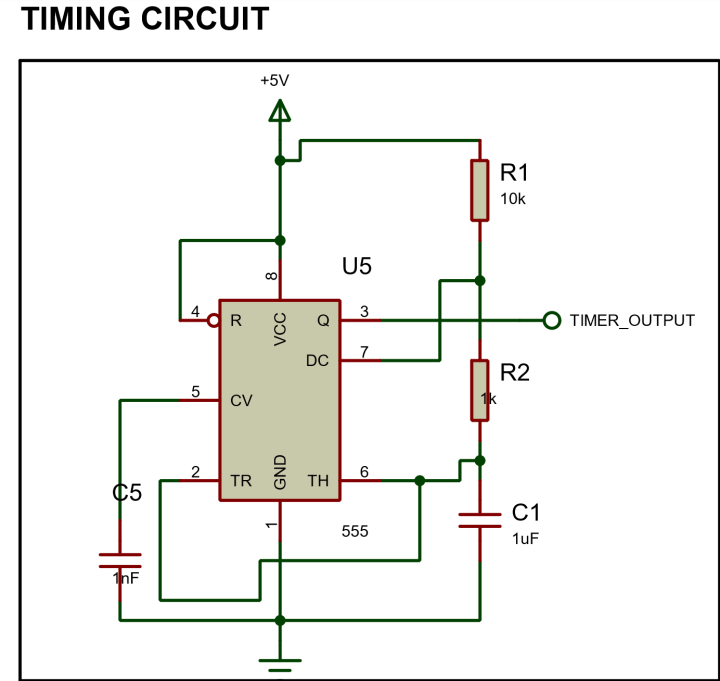
\includegraphics[width=0.65\textwidth]{fig06_timing_circuit_diagram.png}
    \caption{Timing circuit diagram (NE555 astable configuration).}
    \label{fig:timingdiagram}
\end{figure}

\begin{figure}[H]
    \centering
    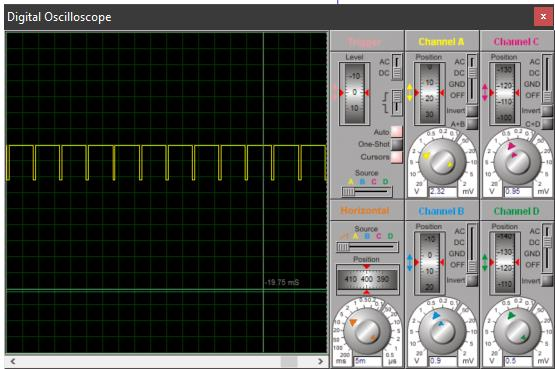
\includegraphics[width=0.80\textwidth]{fig07_oscilloscope_ne555.jpeg}
    \caption{Oscilloscope image of the output signal from the NE555 timer.}
    \label{fig:oscne555}
\end{figure}

% ----- IV. Digital-to-Analogue Signal Converting Circuit ------
\subsection{Digital-to-Analogue Signal Converting Circuit}

The ultrasonic sensor (HC-SR04) outputs a digital signal, while the LM358 operates on analogue
voltages. To interface these components, the digital signal must be converted to an analogue format
using an RC low-pass filter~\cite{circuitcellar2024,electronics_tutorials2024}.

To design the filter, the frequency and voltage levels of the PWM signal from the ultrasonic sensor
must be determined. The appropriate values for $R_5$ and $C_6$ are calculated to achieve a cutoff
frequency of 1~Hz:

\begin{equation}
    f_c = \frac{1}{2\pi RC} \implies 1 = \frac{1}{2\pi \times 1\,\mu\text{F} \times R}
    \implies R = 200\,\text{k}\Omega
    \label{eq:dac}
\end{equation}

\begin{figure}[H]
    \centering
    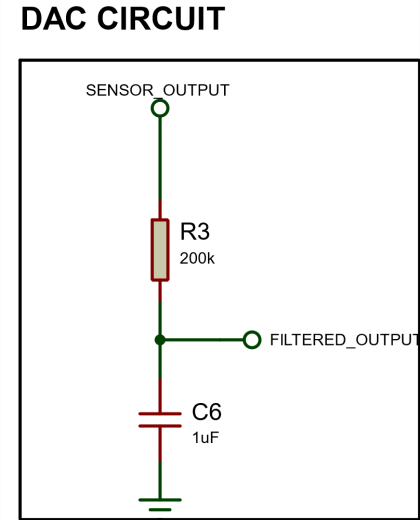
\includegraphics[width=0.55\textwidth]{fig08_dac_circuit.png}
    \caption{DAC (RC low-pass filter) circuit diagram.}
    \label{fig:daccircuit}
\end{figure}

\begin{figure}[H]
    \centering
    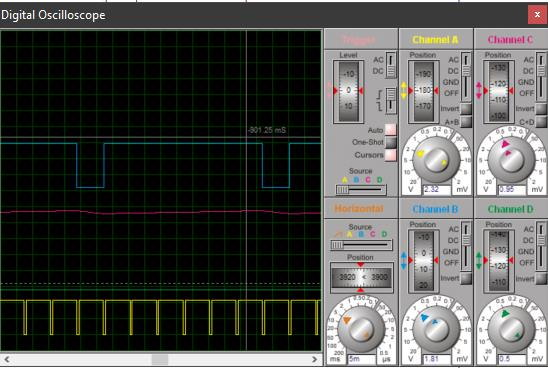
\includegraphics[width=0.82\textwidth]{fig09_oscilloscope_filter.jpeg}
    \caption{Oscilloscope image before and after filtering of the output signal from the ultrasonic
    sensor. The \textbf{blue} PWM signal represents the digital output from the HC-SR04 sensor
    (5~V / 0~V). The \textbf{red} signal represents the converted DC voltage analogue signal.}
    \label{fig:oscfilter}
\end{figure}

As evident, the output is initially in digital form (binary, switching between 5~V and 0~V). The RC
low-pass filter converts this signal to a DC analogue voltage proportional to the measured distance.

% ----- V. Comparator Circuitry --------------------------------
\subsection{Comparator Circuitry}

In this design, an LM358 operational amplifier is configured as a comparator to detect objects within
3-metre and 1-metre ranges using the HC-SR04 proximity sensor. The operational amplifier determines
whether an object is present within the specified distances~\cite{dorf2013circuits,allaboutcircuits2024}.

\begin{enumerate}
    \item \textbf{Reference Voltage Setup:} The reference voltage on the inverting input of the LM358
          op-amp is set slightly below the voltage corresponding to the target distance detected by the
          sensor. For example, if the sensor outputs 2.5~V at 3~metres, the reference voltage is set to
          approximately 2.4~V.
    \item \textbf{Sensing and Comparison:} The voltage from the proximity sensor, which varies with the
          distance of the detected object, is fed into the non-inverting input (positive input) of the
          LM358. As the sensor detects objects, it produces a voltage proportional to the distance.
    \item \textbf{Output Activation:} When the voltage at the non-inverting input exceeds the reference
          voltage at the inverting input, the output of the LM358 goes high (+VCC = 5~V), indicating
          that an object is closer than the threshold distance.
\end{enumerate}

\subsubsection*{Comparator for 3-Metre Detection}

The reference voltage divider is designed as follows:

\begin{equation}
    V_\text{ref} = \frac{R_2}{R_2 + R_1} \implies 3.0 = \frac{R_2}{R_2 + 10\,\text{k}\Omega}
    \implies R_2 = 15\,\text{k}\Omega
    \label{eq:vref3m}
\end{equation}

Reference voltage: $V_\text{ref} = 3.0$~V.

\begin{figure}[H]
    \centering
    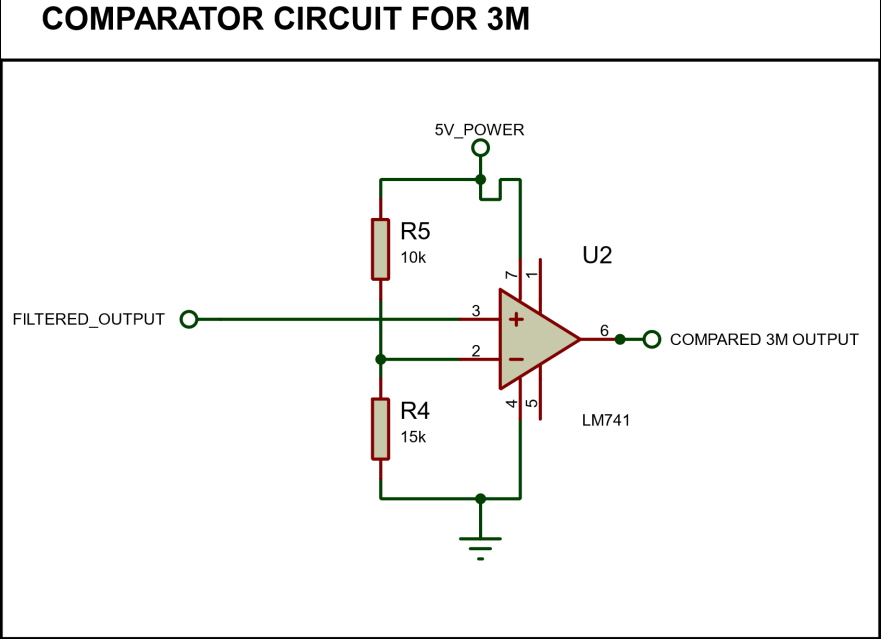
\includegraphics[width=0.65\textwidth]{fig10_comparator_3m.png}
    \caption{LM358 comparator circuit diagram for 3-metre distance alert.}
    \label{fig:comp3m}
\end{figure}

\subsubsection*{Comparator for 1-Metre Detection}

\begin{equation}
    V_\text{ref} = \frac{R_2}{R_2 + R_1} \implies 1.5 = \frac{R_2}{R_2 + 10\,\text{k}\Omega}
    \implies R_2 = 4.3\,\text{k}\Omega
    \label{eq:vref1m}
\end{equation}

Reference voltage: $V_\text{ref} = 1.5$~V.

\begin{figure}[H]
    \centering
    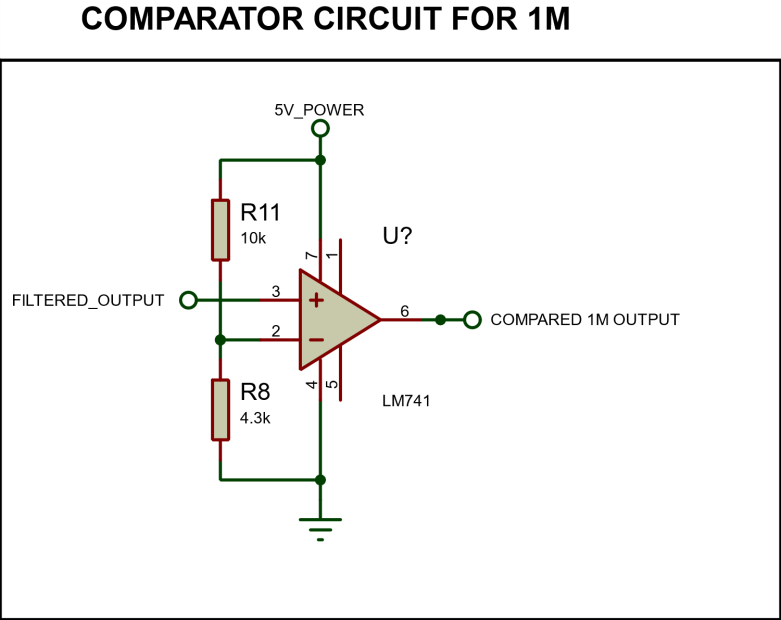
\includegraphics[width=0.65\textwidth]{fig11_comparator_1m.png}
    \caption{Comparator circuit diagram for 1-metre distance alert.}
    \label{fig:comp1m}
\end{figure}

% ----- VI. Output Circuit -------------------------------------
\subsection{Output Circuit}

A relay switch (NT72C) is used to activate the output devices: a DC-operated motor and a piezoelectric
buzzer. When current flows through the relay coil, it generates a magnetic field that attracts the
armature and consequently switches the relay contacts. This mechanism allows the relay to open or close
another circuit based on its normally open (NO) or normally closed (NC)
configuration~\cite{electronics_tutorials2024}. In this design, the normally closed position is connected
to ground and the normally open position is connected to a 5~V power supply.

The output circuit feedback devices are:
\begin{itemize}
    \item A 5~V DC-operated motor and a piezoelectric buzzer, activated when the 1-metre LM358
          comparator detects an object.
    \item A DC-operated piezoelectric buzzer only, activated when the 3-metre LM358 comparator
          detects an object.
\end{itemize}

\begin{figure}[H]
    \centering
    \begin{subfigure}[t]{0.48\textwidth}
        \centering
        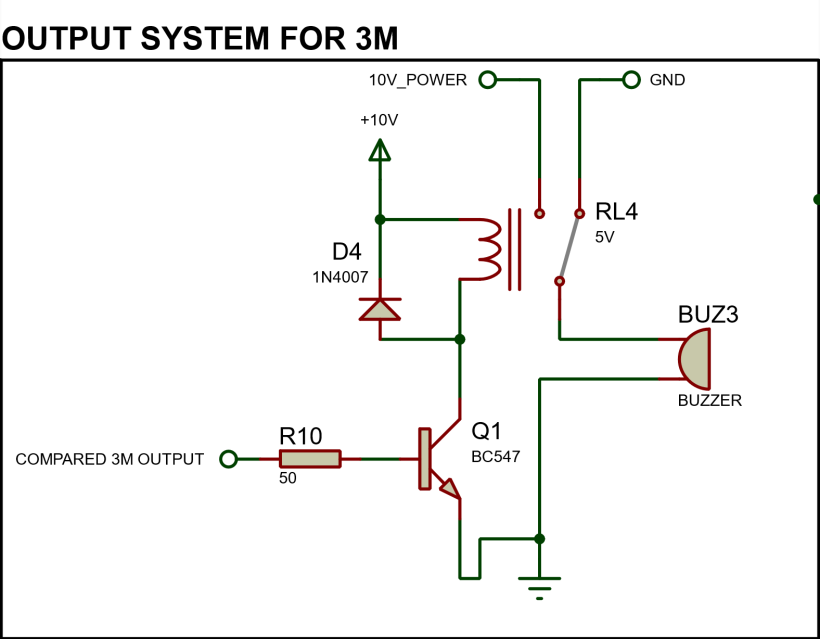
\includegraphics[width=\textwidth]{fig13a_output_3m.png}
        \caption{Output circuitry for the 3-metre detection system.}
        \label{fig:output3m}
    \end{subfigure}
    \hfill
    \begin{subfigure}[t]{0.48\textwidth}
        \centering
        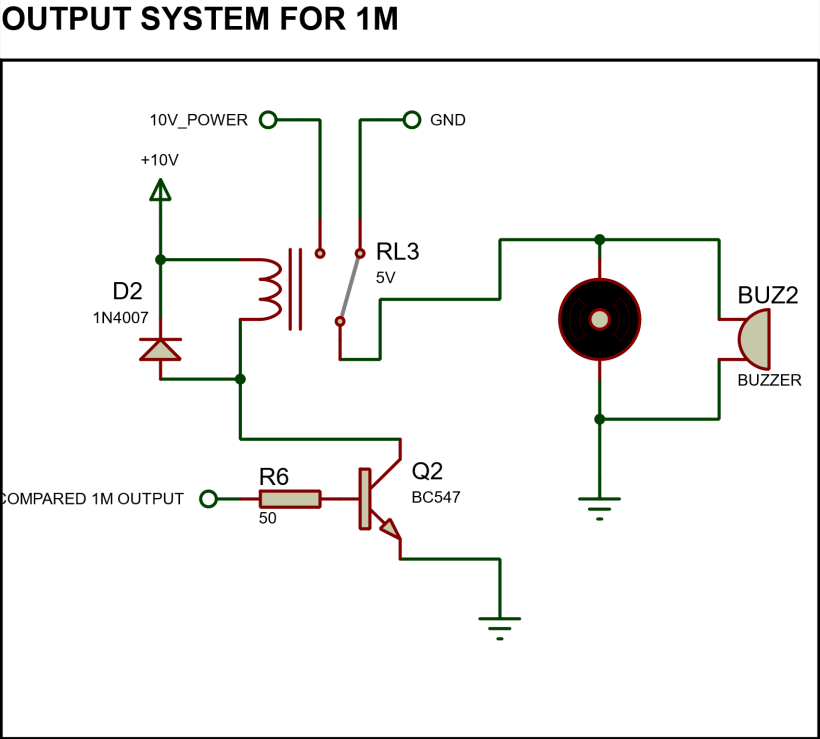
\includegraphics[width=\textwidth]{fig13b_output_1m.png}
        \caption{Output circuitry for the 1-metre detection system.}
        \label{fig:output1m}
    \end{subfigure}
    \caption{Output circuit diagrams for both detection thresholds.}
    \label{fig:outputcircuits}
\end{figure}

% =============================================================
\section{Results and Analysis}
% =============================================================

The device is designed to alert users as they approach obstacles from a specific distance. Initially,
when an obstacle is detected 3~metres away, the device emits a sound from a buzzer to alert the user.
As the user moves closer to the obstacle, reaching a distance of 1~metre, the device provides an
additional alert through both a vibration from a DC motor and a sound from the buzzer. This
dual-feedback system ensures that users are adequately informed about their proximity to nearby
objects, enhancing their ability to navigate their environment safely.

\subsection*{Prototype}

A working simulating prototype was developed in TinkerCad software and subsequently simulated on
Proteus.

\begin{figure}[H]
    \centering
    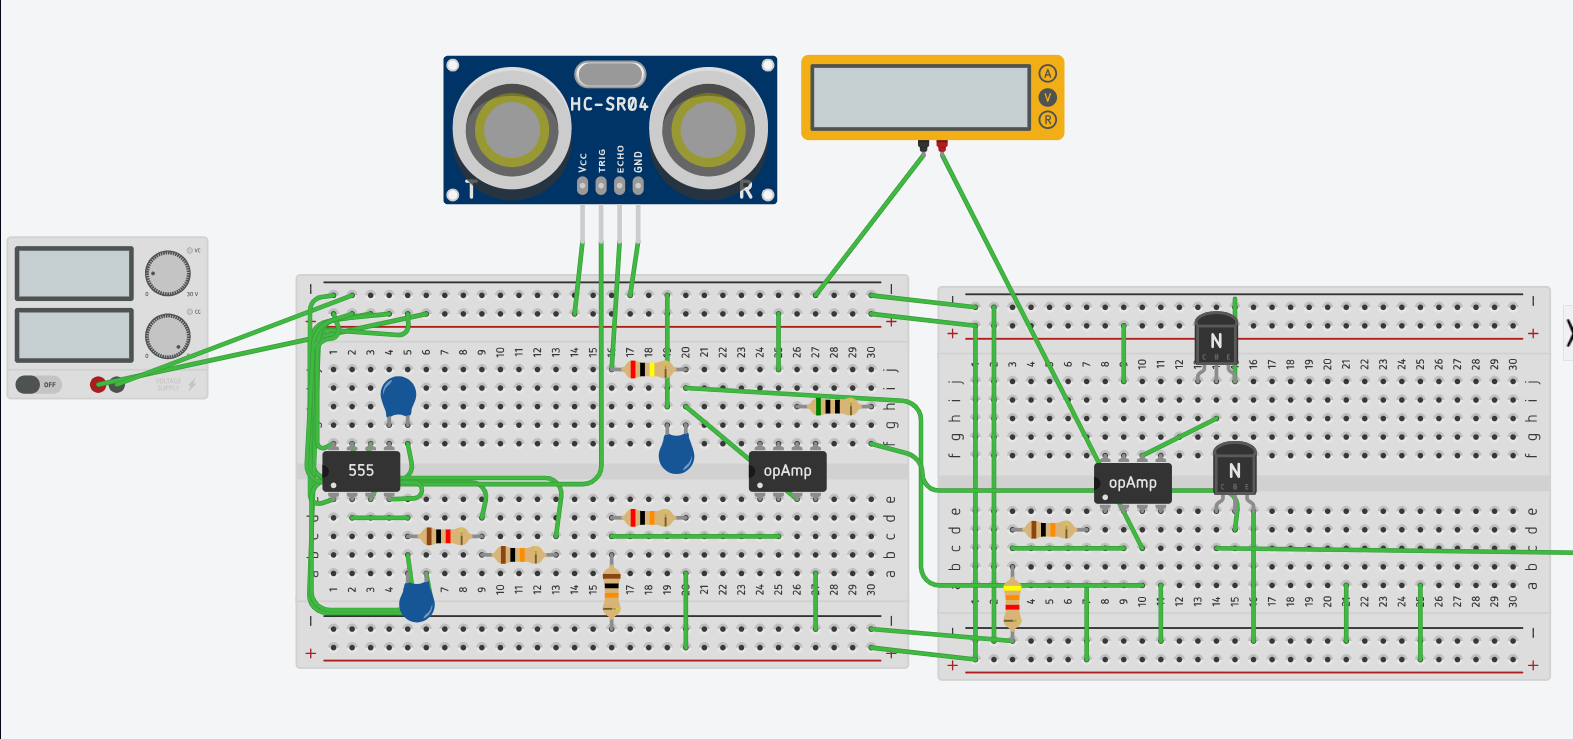
\includegraphics[width=0.85\textwidth]{fig14a_tinkercad_sensing.png}
    \caption{TinkerCad prototype showing the sensory, timing, and comparator circuits.}
    \label{fig:tinkercad_sensing}
\end{figure}

\begin{figure}[H]
    \centering
    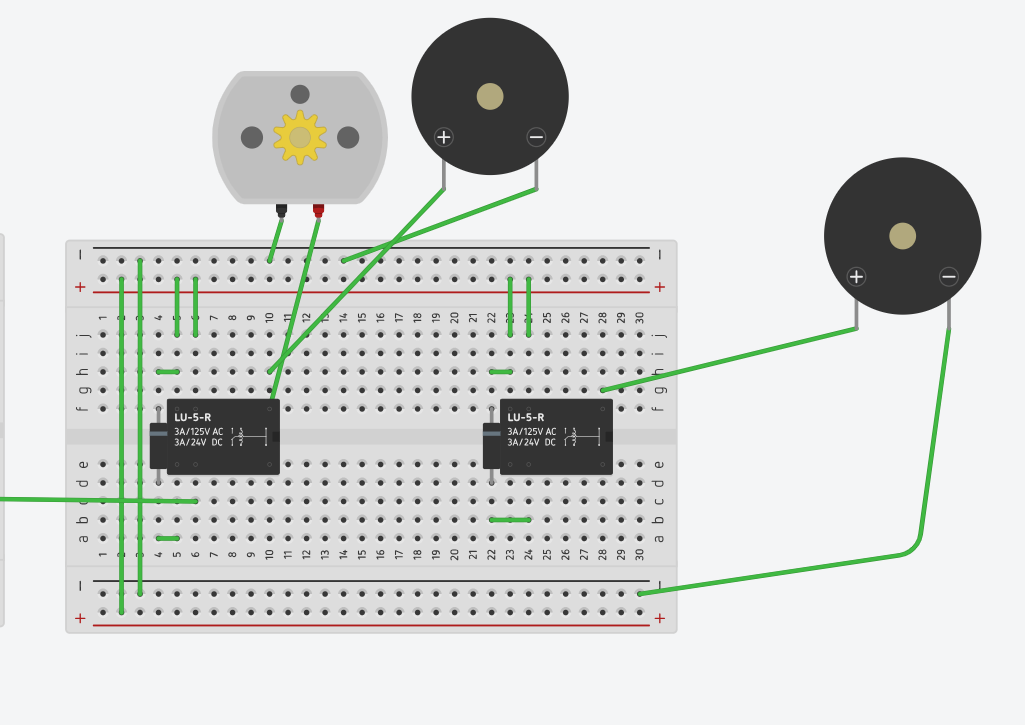
\includegraphics[width=0.75\textwidth]{fig14b_tinkercad_output.png}
    \caption{TinkerCad prototype showing the output circuit.}
    \label{fig:tinkercad_output}
\end{figure}

\begin{figure}[H]
    \centering
    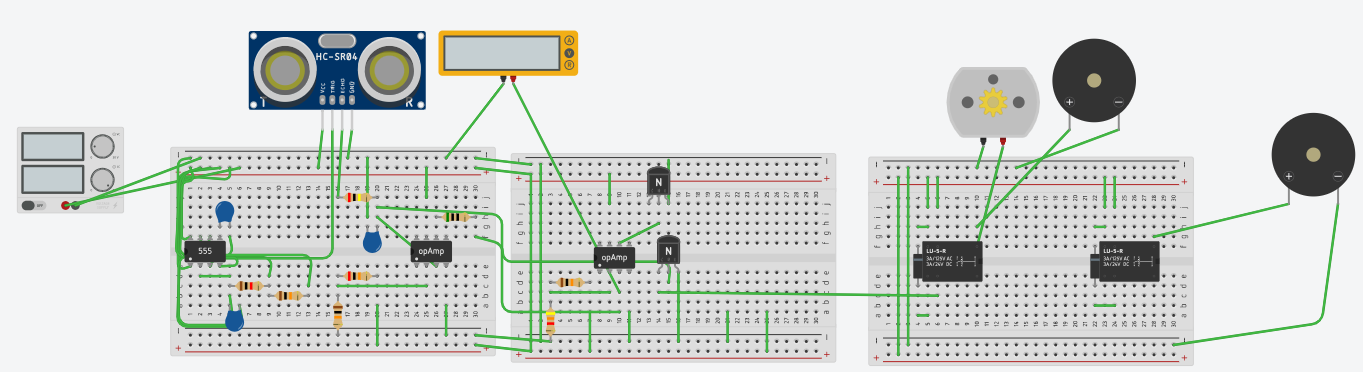
\includegraphics[width=0.95\textwidth]{fig14c_tinkercad_overview.png}
    \caption{Overview of the complete TinkerCad prototype of the design.}
    \label{fig:tinkercad_overview}
\end{figure}

\begin{figure}[H]
    \centering
    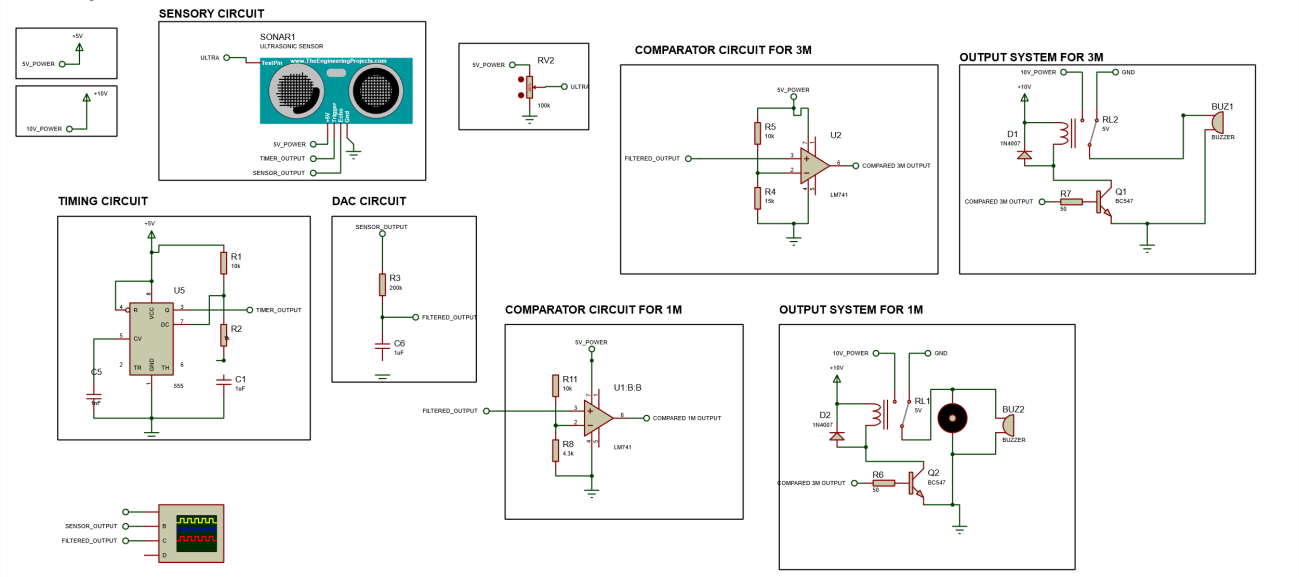
\includegraphics[width=0.95\textwidth]{fig15_proteus_simulation.png}
    \caption{Proteus simulation of the complete circuit.}
    \label{fig:proteus}
\end{figure}

\subsection*{Testing}

\subsubsection*{Off-State}

When the system is powered up, the NE555 timer receives power and begins generating a square wave
at 250~Hz. The HC-SR04 starts generating pulse waves of 8 oscillations. When there is no signal input
to the sensor, no voltage drops are generated and the RC low-pass filter outputs 0~V at the node. This
0~V is conducted into both comparators (LM358). Since the reference voltage is higher than the voltage
at the non-inverting terminal, the output voltage from both op-amps is 0~V. Consequently, the current
at the base of the NPN transistors (BC547) is zero (cutoff state), no current flows at the collector, and
the relay switch remains in the normally closed position. No current flows into the buzzer or motor, and
no output feedback is produced.

\begin{figure}[H]
    \centering
    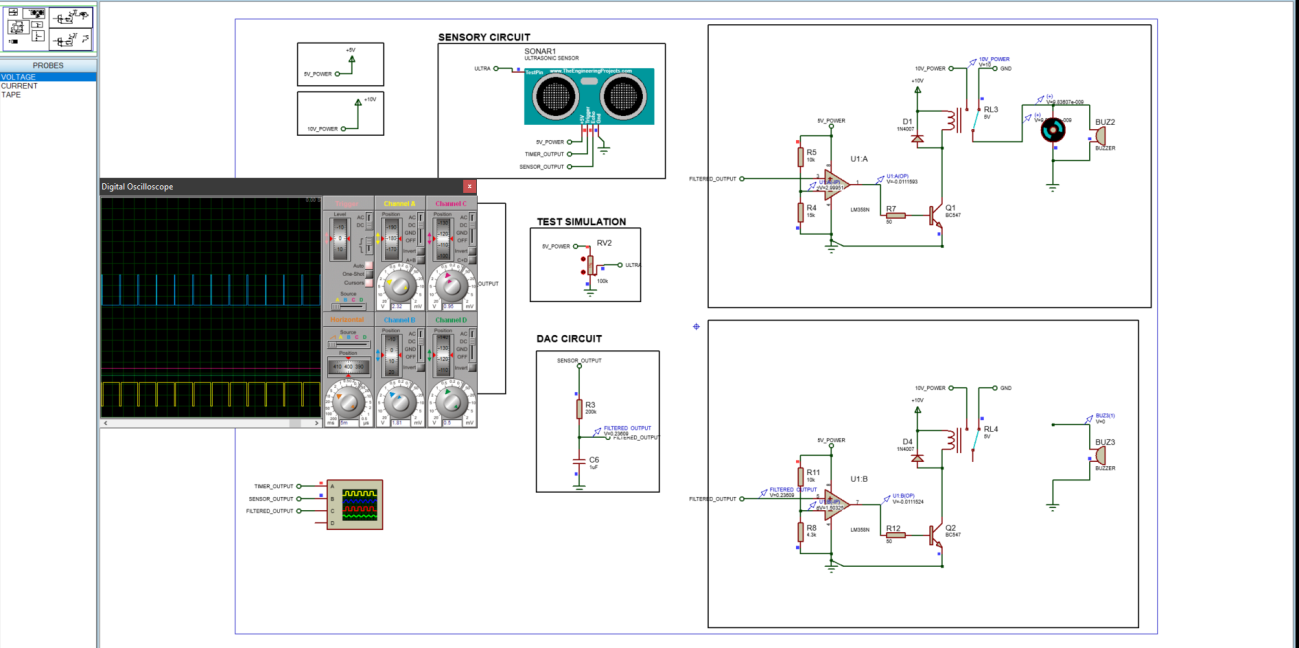
\includegraphics[width=0.95\textwidth]{fig16_offstate_voltages.png}
    \caption{Diagram showing the different voltages at different areas of the circuit in the Off-State.}
    \label{fig:offstate}
\end{figure}

\subsubsection*{On-State}

When the sensor detects an object and receives a trigger input, it generates a voltage in digital form.
This voltage is converted to an analogue DC voltage via the RC low-pass filter and is conducted into
the non-inverting terminals of the op-amps (LM358). When the voltage at the non-inverting terminal
exceeds the reference voltage at the inverting terminal, the output of the LM358 goes to 5~V (VCC).
This 5~V forward-biases the NPN transistor, allowing current to flow through the relay coil. The relay
energises and switches from normally closed to normally open, activating the output devices. The
specific output depends on the measured distance:

\begin{itemize}
    \item \textbf{3-metre detection:} The buzzer produces sound.
    \item \textbf{1-metre detection:} Both the buzzer and DC motor are activated (sound and vibration).
\end{itemize}

The oscilloscope readings confirm that larger distances produce larger pulse widths, corresponding to
higher analogue voltage levels.

\begin{figure}[H]
    \centering
    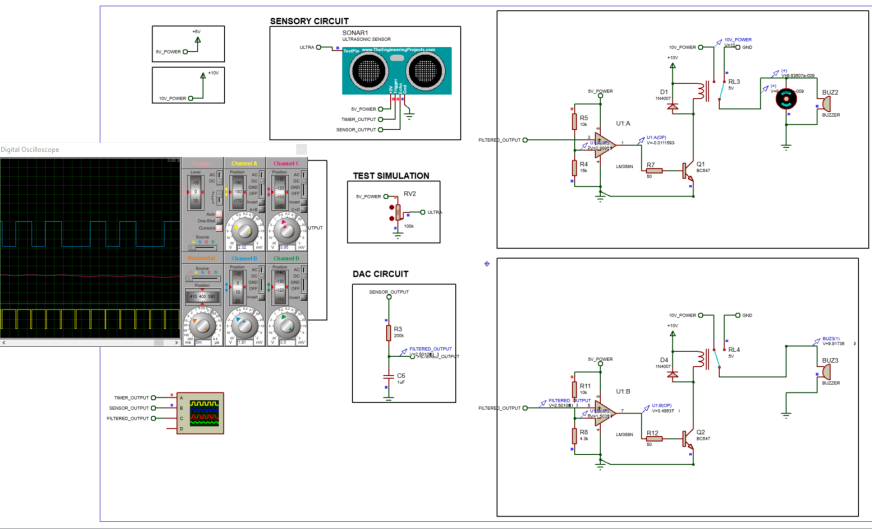
\includegraphics[width=0.92\textwidth]{fig17_onstate_1m.png}
    \caption{Diagram showing the circuit response when an object is detected at 1-metre range.}
    \label{fig:onstate1m}
\end{figure}

\begin{figure}[H]
    \centering
    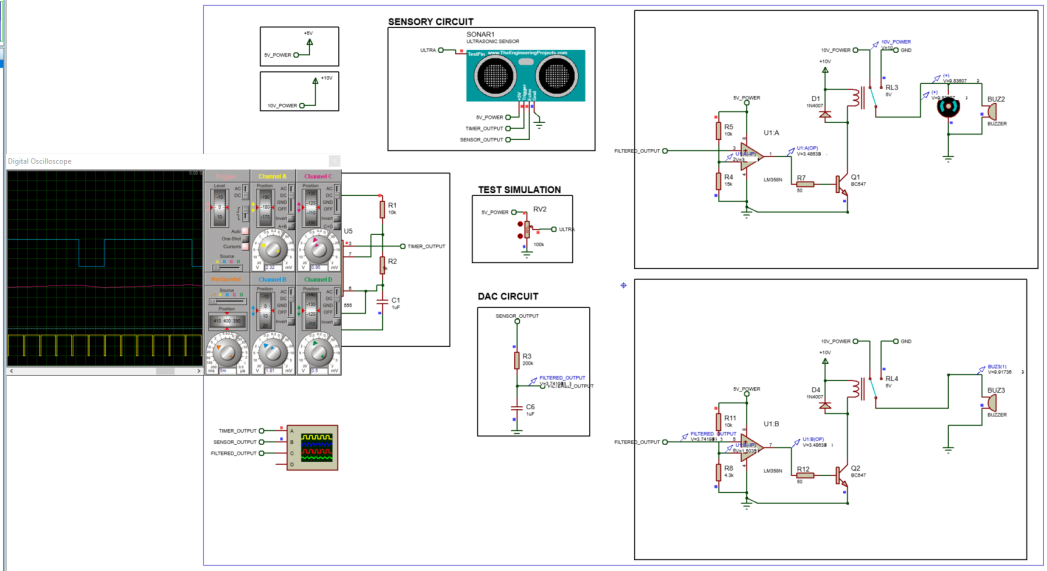
\includegraphics[width=0.92\textwidth]{fig18_onstate_3m.png}
    \caption{Diagram showing the circuit response when an object is detected at 3-metre range.}
    \label{fig:onstate3m}
\end{figure}

% =============================================================
\section*{Conclusion}
\addcontentsline{toc}{section}{Conclusion}
% =============================================================

This research paper presents the design, simulation, and analysis of an aiding system for visually
impaired individuals using a handheld, rechargeable stick which operates on proximity sensors. The
main objective was to detect objects at two distinct distances: 1~metre and 3~metres. The device is
handheld and rechargeable, and intended for daily use. The system was designed to be easy to use.

This project addresses problems faced by visually impaired individuals such as requiring secondary
personnel for mobility and navigation in unknown surroundings. Users will be able to navigate unknown
spaces with a navigation system that detects obstacles well in advance. This design demonstrates
significant potential for further improvement; challenges encountered during implementation can be
overcome with the appropriate time and resources.

% =============================================================
\bibliographystyle{IEEEtran}
\bibliography{references}
% =============================================================

\end{document}
